\section{Понятия реляционной теории}
\indent Для организации и теоретического обоснования описанного ранее хранилища, использовалась теория реляционных баз данных.
\indent Теория реляционных баз данных оперирует понятиями отношения (relation, от которого и пошло само название теории и баз данных основанных на ней), атрибута, домена и кортежа.

\begin{figure}[ht]
	\centering
	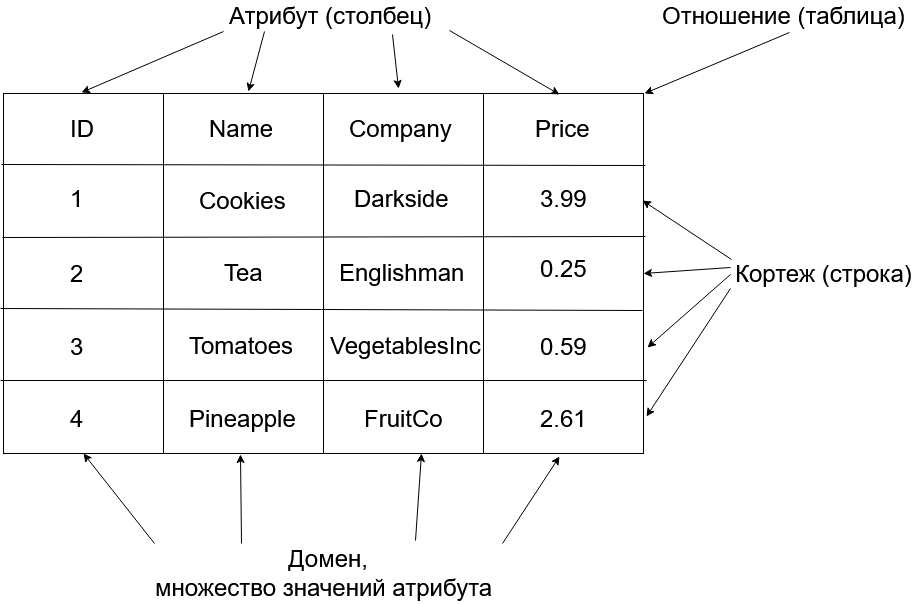
\includegraphics[width=\linewidth]{pics/databaseExample.png}
	\caption{Понятия реляционной базы данных}
	\label{fig:dbExample}
\end{figure}

\indent Атрибут - именованный столбец отношения.
В пределах одного атрибута все значения должны быть одного типа данных, то есть принадлежать одному домену.\\
\indent Домен - тип данных, множество всех допустимых значений атрибута.\\
\indent Кортеж - упорядоченный набор из N элементов, где N - это число атрибутов отношения.
Иначе говоря, кортеж - это строка или запись таблицы.\\
\indent Отношение - множество упорядоченных N-кортежей.
Другими словами отношение - это двумерная (плоская) таблица, состоящая из столбцов и строк - атрибутов и кортежей (см. \ref{fig:dbExample}).\\
\indent Также вводится понятие целостности по ссылкам - 
\todo{добавить определение внешнего ключа и целостности по ссылкам}

\section{Обоснование}
\indent Пусть заданы два отношения $R_1$ и $R_2$, такие что:
% \begin{center}
\begin{multline*}
		R_1 = <name, version, ...>\\
		R_2 = <FK(R_1, name), version, ...>
\end{multline*}
% \end{center}

\indent $FK(R, a)$ - внешний ключ, ссылающийся на атрибут $a$ на отношения $R$, тогда:
\todo{выровнять}
\begin{multline*}
	\forall name \in R_1.name : \forall v_1 \in R_1.version v_2 \in R_1.version: v_1 \neq v_2 : \\
		S_{v_1} = \sigma_{name, v}(R_1 \bowtie_{name = R_2.name, v_1 \leq R_2.version}R_2) \\
		S_{v_2} = \sigma_{name = name, F_{MAX(version)} = v}(R_1 \bowtie_{name = R_2.name, v_2 \leq R_2.version}R_2) \\
		S_{v_1} \cap S_{v_2} = ???
\end{multline*}

\todo[inline]{Доказать и можно вводить оператор}

\begin{equation}
	\label{eq:versJoin}
	R_1\overrightarrow{\bowtie} R_2 \Leftrightarrow \pi_{*, F_{MAX(R_1.version)}}(\sigma_{R_1.version \leq R_2.version}(R_1 \bowtie_{R_1.name = R_2.name}R_2))
\end{equation}

\indent Формула \ref{eq:versJoin} отражает эквивалентность ``версионного пересечение'' (слева) и реляционного выражения справа.
Под знаком ``*'' понимается проекция всех атрибутов из полученного отношения.

\todo[inline]{монотонность версий}
